\subsection{Historique, acteurs et objectifs}

Dans cette section, il s'agit d'examiner plus en profondeur l’histoire et l’origine des choix architecturaux et technologiques déterminés par le projet \pense. Il nous paraît tout d’abord en effet essentiel de replacer l’émergence de ce projet dans un contexte historique, scientifique et institutionnel afin d’en cerner la genèse, la trajectoire et les ambitions. Porté par le Service numérique de la recherche, qui en assure la facette technique, le projet a la caractéristique de dépasser le simple cadre du Département des Etudes et de la Recherche (dont dépend le SNR), pour être placé sous l’égide des deux départements fondamentaux de l’\inha, dont le Département de la Bibliothèque et de la Documentation. 

\subsubsection{A la genèse du projet : la constitution d’un service numérique de la recherche}
\newline
\textbfit{L’INHA : Une institution issue d’un projet ancien et placée au carrefour des mondes scientifique et culturel pour la valorisation de l’histoire de l'art comme discipline}

L'Institut national d’histoire de l’art (INHA) a vu le jour en 2001, mais ses racines sont plus anciennes – citons la proposition de l’historien de l’art Jacques Thuillier en 1973 de la création d’un institut national entièrement consacré à la recherche dans ce domaine d’étude, formalisée en 1983 par un autre grand historien de l’art, André Chastel\footcite{inha_presentation_nodate}. Etablissement situé au croisement entre le monde de la recherche et de la culture, comme le suggère la double tutelle ministérielle dont il est issu, il a pour mission de promouvoir la recherche scientifique dans le domaine de l’histoire de l’art, tout en valorisant ses propres fonds, puisque l’Institut est également un lieu de conservation à travers sa bibliothèque.
L'\inha s'articule autour de deux grands départements : le Département des études et de la recherche (DER) et le Département de la bibliothèque et de la documentation (DBD), dont les missions se veulent complémentaires\footcite{inha_organisation_nodate}. 
Le Département des Études et de la Recherche (DER) est la branche de l’INHA dédiée à la production et à la coordination des recherches scientifiques. Structuré autour de huit domaines de recherche, répartis entre domaines périodiques et thématiques, le DER dirige des programmes qui répondent à deux objectifs principaux : d’une part, la création de ressources scientifiques pour les historiens de l’art et d’autre part, la valorisation des fonds bibliographiques de l’institut\footcite{inha_departement_nodate}.
\newline
\textbfit{La naissance du Service numérique de la recherche}\\

Le DER disposait, depuis 2001, d’une \cid, qui avait pour mission d’accompagner les chercheurs dans la gestion et la production de ressources numériques pour les programmes scientifiques menés par le département et ses partenaires. La \cid gérait également l’administration de la plateforme AGORHA, un outil de mutualisation des bases de données développées par l’institut\footcite{courtin_rapport_2019}, qui centralise à l’heure actuelle plus d’une cinquantaine de bases. 
En 2019, notamment sous l’impulsion d’Antoine Courtin, alors à la tête du service, la cellule s’est transformée en un Service numérique de la recherche (SNR), dans le but de renforcer l’appui fourni aux chercheurs dans la gestion des données numériques, tout en adaptant les infrastructures aux besoins croissants en matière de production et de diffusion des ressources numériques\footcite{inha_service_nodate}.
Le \snr est aujourd’hui structuré en différents pôles spécialisés, chacun ayant des missions spécifiques : la curation des données de la recherche, l’édition numérique enrichie, la gestion documentaire numérique et le conseil stratégique. L’équipe comprend des ingénieurs de recherche, des moniteurs étudiants ainsi que des chargés de ressources documentaires et numériques. Ce service accueille régulièrement des chercheurs, doctorants et stagiaires qui participent activement à ses projets\footcite{nurra_presentation_2023}.
\newline
\textbfit{Les précurseurs du projet PENSE}\\

Le projet \textif{Digital Montagny}, dirigé par Martine Denoyelle, Delphine Burlot et Murtha Baca et réalisé en collaboration avec le Getty Research Institute, constitue l’un des exemples des projets d’édition critique porté par la \cid, en 2014-2015\footcite[p.13]{courtin_rapport_2019}. 
Portant sur l’édition d’un album de dessins du peintre Élie-Honoré Montagny (1782-1864), \textit{Recueil d’Antiquités}, documentant les monuments antiques conservés à Naples et Rome au début du XIXe siècle\footcite{inha_digital_nodate}, il était appuyé sur le système de gestion de contenu (\cms) \textit{Drupal}, ce qui témoigne d’une approche distincte de celle choisie postérieurement pour \pense, mais poursuivie avec le \textif{Digital Muret}. 
Ce dernier, quant à lui toujours accessible en ligne, propose une édition critique des dessins de Jean-Baptiste Muret (1795-1866), accompagnée d’une attention portée à la sémantisation des contenus, et à la constitution parcours éditoriaux\footcite[p.49]{courtin_rapport_2019} permettant à tous les publics de saisir la richesse de la réunion du fonds documentaire constitué par les dessins de Muret avec la collection d’objets archéologiques rassemblés par ce dernier, les deux étant mis en regard\footcite{noauthor_a_nodate}.

Ce projet faisait appel à des outils de crowdsourcing pour enrichir le contenu\footcite[p.53]{courtin_rapport_2019}. Une dimension collaborative facilitée par le choix du \cms \textit{Omeka S} (repris, au même titre que les efforts de sémantisation et de liage des contenus, pour la refondation d’AGORHA en 2021), comme le souligne \citeauthor{chateau-dutier_editions_2021} en formulant une comparaison entre le Digital Muret et une autre édition numérique présentant des caractéristiques similaires, le \textit{Pietro Mellini’s inventory in verse}, ou \textit{Digital Mellini} (2015), porté par le Getty Research Institute et l’Université de Malaga, et lui appuyé sur \textit{Drupal}, puisque conçu avant l’arrivée du \cms \textit{Omeka S}\footcite{daniel_digital_2014}.

Bien que le projet \pense, issu du travail d’acteurs différents, ne s’inscrive pas directement en héritage de ces projets d’édition numérique antérieurs en ce qu’il ne s’appuie notamment pas directement sur les mêmes infrastructures technologiques que le \textit{Montagny} ou le \textit{Muret} (abandon des \cms…), il en partage néanmoins les grandes étapes méthodologiques. En effet, les trois projets suivent un processus similaire : gestion documentaire, curation des données et exposition sous la forme d’une interface qui puisse être facilement prise en main, voire qui soit facilement appropriée par les utilisateurs/lecteurs\footcite{colonna_digital_2024}.

\subsubsection{Une impulsion : l’acquisition du fonds Barye en 2018}

C’est l’acquisition en 2018 du fonds Barye, correspondant aux archives d’Antoine-Louis Barye (1795-1875), sculpteur et peintre animalier, par la bibliothèque de l’\inha qui va véritablement donner l’impulsion au projet \pense. Ce fonds relativement volumineux, qui comprend environ 350 pièces, principalement des correspondances, mais aussi des documents plus divers liés à l'activité de Barye, couvre une période particulièrement longue, s’étendant de 1819 à 1912. Dès 2019, l’INHA prend la décision de compléter ce fonds par une édition numérique, inscrivant cette entreprise dans une stratégie plus large de valorisation des collections patrimoniales de l’institut\footcite{inha_edition_nodate}. 
C’est dans ce contexte que naît le projet \pense, concrétisé début 2020 avec le recrutement d’un ingénieur de recherche spécialement chargé de sa mise en œuvre.

Le projet \pense, dès ses premières étapes, se distingue par une approche pragmatique inspirée de la méthodologie Agile. Comme le souligne Jean-Christophe Carius dans un entretien réalisé en juillet 2024 dans le cadre du stage, contrairement aux démarches théoriques souvent longues et préparatoires qui ont tendance à caractériser ce type de projets, le choix est fait de passer rapidement à des applications concrètes, en intégrant dès le départ le recours à des outils numériques avancés. Ce positionnement permet d’amorcer les premières réalisations sans attendre un cadre théorique définitif, donnant au projet un caractère modulable dès ses débuts. En effet, la première année de mise en œuvre, deux projets pilotes sont développés : l’édition numérique du fonds Barye et, neuf mois plus tard, celle du fonds Karbowsky. 
\newline
\textbfit{L’édition \emph{Karbowsky}, vers une diversification des corpus traités par PENSE}\\

Ce second corpus, qui repose principalement sur un ensemble d’œuvres iconographiques, est choisi pour diversifier les types de documents traités dans le cadre de \pense et d’éprouver la capacité du projet à l’adaptation. Il s’agissait de valider l'extension de ses fonctionnalités au-delà des textes, comme l’indique Jean-Christophe Carius\footcite{carius_ledition_2022}. 
Ce projet repose, lui, sur la numérisation d'un fonds plus modeste en terme de volumétrie : il s’agit de réaliser l’édition numérique de 31 aquarelles réalisées par le décorateur Adrien Karbowsky (1855-1945), figurant des vues détaillées de l'hôtel particulier de Jacques Doucet, situé au 19 rue Spontini à Paris. Ces œuvres, exécutées en 1906, représentent les pièces de cet hôtel, où les objets de collection sont, de par la finesse de l’exécution picturale, aisément identifiables\footcite{carius_ledition_2022}.

Un aspect remarquable à mentionner concernant ce projet, réside dans le choix plutôt innovant d’inclure une reconstitution virtuelle de l'hôtel particulier de Doucet. Il est donc ainsi possible de « plonger » dans les aquarelles de Karbowsky, offrant au lecteur/récepteur une expérience immersive et interactive\footnote{Accessible à cette adresse : https://karbowsky.inha.fr/Experience3D.}, dimension qui n’est pas toujours explorée dans les projets d’édition numérique plus traditionnels.
\newline
\textbfit{\emph{Barye} et \emph{Karbowsky}, deux projets pilotes}\\

Ces deux projets pilotes ont joué un rôle central dans la définition des orientations techniques et méthodologiques de \pense, en modelant à la fois une approche technologique et pratique (gestion de projet). Les choix logiciels effectués pour ces premières éditions ont ainsi servi de modèle, ou du moins de point de départ, pour les projets suivants, offrant une sorte de feuille de style commune. Toutefois, il faut souligner chaque projet conserve ses propres spécificités. 

Les projets Barye et Karbowsky partagent bien, en effet, des fondements techniques similaires, s’appuyant notamment sur l’utilisation d’une base \xml native et de l’outil Transkribus, permettant la reconnaissance et la transcription automatisée des documents (utilisé pour la transcription et la segmentation manuelle dans le cadre de \pense). 
Une autre caractéristique commune est l'utilisation de la bibliothèque JavaScript \textit{Datatable}, qui permet la création d'interfaces web dynamiques structurées grâce à la constitution de tableaux \html dissimulés dans les pages, permettant une manipulation et une exposition plus facile des données. Cependant, des différences sont à noter entre les deux projets : l’édition du fonds Karbowsky, par exemple, s’appuie sur la base AGORHA, ce qui n’est pas le cas de l’édition \textit{Barye}.

\subsection{Architecture logicielle et choix techniques}

\subsubsection{Des éditions numériques appuyées sur la technologie XML}

Le choix d'utiliser \xml comme base technique pour le projet \pense n’est pas surprenant dans le domaine de l'édition numérique savante. Le format \xml est généralement privilégié pour la structuration et la description des documents textuels pour son architecture arborescente permettant une meilleure navigation dans les données (facilitée par le langage de requête XPath notamment). Mais surtout, il permet d’intégrer aisément le format \tei, devenu standard pour l’édition numérique dans les projets francophones et anglophones notamment. Ce choix s’accompagne presque naturellement (même s’il est possible, bien que moins aisé, de gérer des données \xml avec des bases relationnelles de type SQL) de l’utilisation de bases de données XML natives, dites « bases de données orientées document » qui permettent de stocker et de rechercher des documents complexes en conservant leur dimension arborescente, sans avoir à les fragmenter en tableaux ou en relations multiples, comme c'est le cas avec SQL. 

Le système de gestion de bases de données \textit{BaseX} a été retenu pour le stockage des données XML dans le cadre de \pense, en raison de ses performances reconnues dans la gestion de grandes bases de données documentaires\footcite{truica_forgotten_2021} – il a également été préféré à son homologue \textit{eXist-DB}, jugée moins ergonomique et intuitif, en raison notamment d’une meilleure connaissance par l’ingénieur en charge du développement du projet.  
Initialement développé en 2005 dans le cadre d’un projet de recherche, \textit{BaseX} a rapidement évolué vers un outil open source à part entière, intégrant un processeur XPath/XQuery\footcite{noauthor_BaseXgui_2019}. Il est conçu pour être à la fois un gestionnaire de bases de données et un moteur d’applications web, ce qui permet à l’équipe du projet \pense de déployer des interfaces interactives sans avoir à passer par des systèmes de gestion de contenu (\cms) comme \textit{Omeka}, qui reposent sur des bases de données relationnelles et dont le choix aurait nécessité un reformatage des données voire une refondation totale de la chaîne de traitement.

Le choix de \textit{BaseX} s’explique donc naturellement par la structure même des données à traiter, mais aussi par la volonté de l’ingénieur en charge de s’affranchir des limites des \cms standards.

\subsubsection{Un soin apporté au design d’interfaces}

Sur le plan du design graphique, le projet \pense s’est distingué par une grande attention portée à l’élégance, l’intelligibilité et à l’ergonomie, sans pour autant adopter une charte graphique stricte. L’objectif principal était d’assurer par des choix formels une expérience utilisateur agréable et fluide, plutôt que de définir une identité visuelle forte. Cependant, le choix des polices typographiques, par exemple, demeure principalement dicté par les standards graphiques de l’INHA, témoignage d’une recherche de cohérence graphique avec les autres contenus produits par l’institution sur le Web. Les inspirations graphiques du projet, selon l’ingénieur en supervisant le développement, sont à rechercher du côté d'autres projets similaires, comme \textit{Architrave}, projet consacré à l’art et l’architecture à Paris et Versailles à l’époque baroque dans les récits de voyageurs allemands\footcite{noauthor_architrave_nodate} ou \textit{Der Sturm}, consacré quant à lui à l'édition numérique de la revue d’avant-garde expressionniste éponyme, avec un soin particulier apporté à une certaine fidélité visuelle aux documents originaux\footcite{noauthor_startseite_nodate}.

L’importance du design est également manifeste dans les diverses formes de visualisation des documents proposées par \pense, notamment pour le fonds Barye. Il s’agit ici, non pas de s’intéresser au design d’interface dans sa recherche d’ergonomie et de praticité, mais de réfléchir à des manières d’apprécier et de mettre en exergue la matérialité de l’archive, aspect que l’on pourrait croire mis de côté voire invisibilisé par la dimension numérique de l’édition. Cette représentation graphique du document objet de l’édition dans son aspect d’objet matériel, véritable visualisation permettant de restituer la « multi-dimensionalité de l’archive » \footcite[p.83]{chateau-dutier_editions_2021}, est plébiscitée par Anthony Masure\footnote{A propos des choix de design du projet \textit{Collecta}, auquel il a participé, in \footcite[16ème minute]{masure_design_2017}} comme un moyen d’offrir au chercheur consultant l’interface d’appréhender le document d’une manière différente de celle adoptée dans le cadre du traitement scientifique, en se représentant ses proportions et sa « physicalité », voire en restituant un peu du « goût de l’archive » cher à Arlette Farge (conceptualisant la relation intime de l’historien à l’objet-archive constitué par les sources primaires). 
Dans le cas de Barye, il a été fait un choix de représenter, selon plusieurs formes de visualisations différentes, le fonds sous sa forme matérielle, avec une dimension interactive plus ou moins prononcée selon les technologies utilisées. 
Quatre types de représentations graphiques distinctes ont été ainsi développées au fil du temps, chacune répondant à des besoins spécifiques en termes de visualisation des données. 
Nous allons les présenter ici : 

\begin{figure}[h] 
        \centering 
        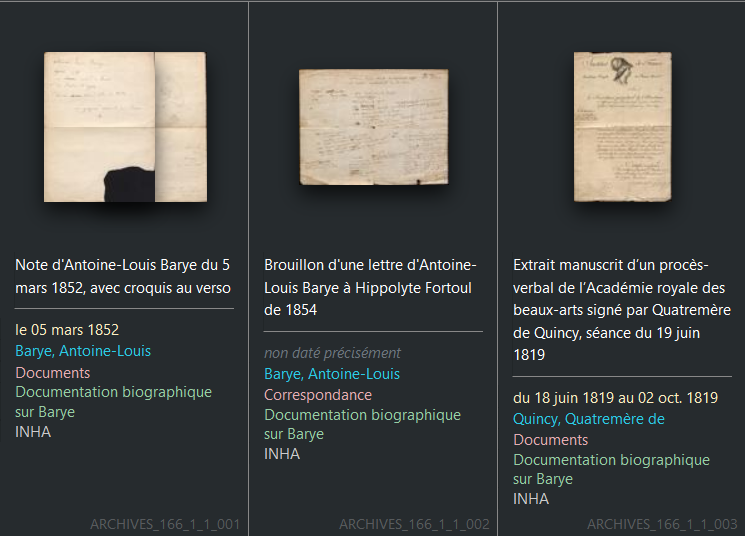
\includegraphics[width=0.8\textwidth]{barye_design_a_plat} 
        \caption{Visualisation « à plat » des documents.} 
        \label{fig:visualisation-plat} 
\end{figure}

La première forme, dite à plat, présente les pages des documents numérisés de manière juxtaposée, permettant ainsi une vue d'ensemble du corpus\footnote{Disponible à l’adresse suivante : https://barye.inha.fr/corpus}. Cette approche, simple, présente l'inconvénient de ne pas rendre compte de toute la matérialité des documents (trois dimensions, volumétrie…). 

\begin{figure}[h] 
        \centering 
        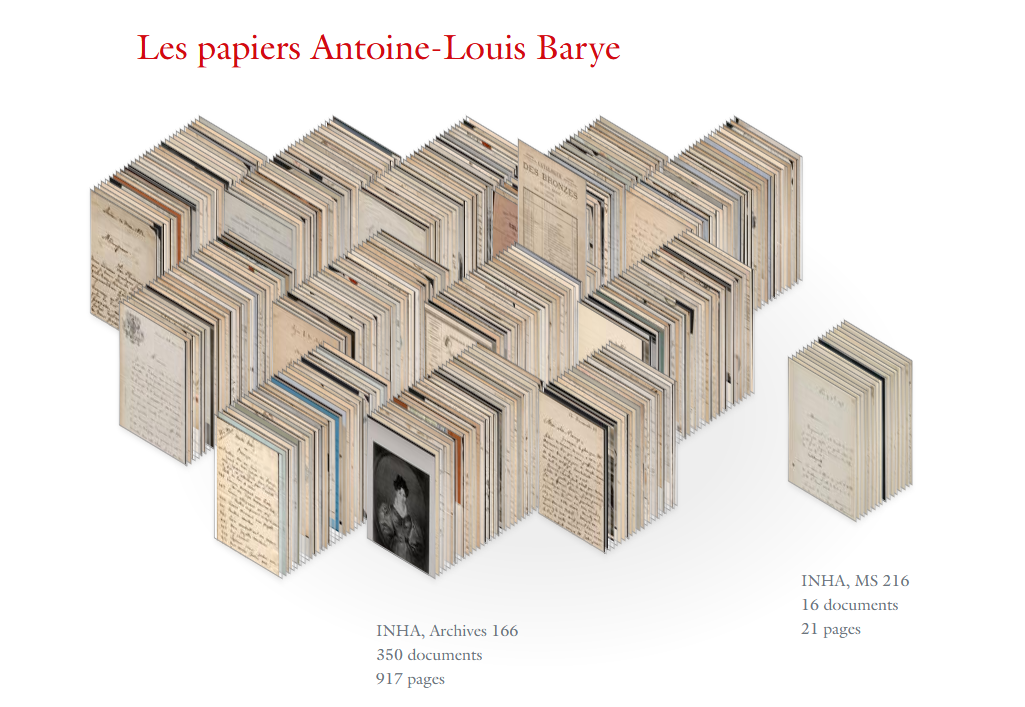
\includegraphics[width=0.8\textwidth]{barye_design_isometrique } 
        \caption{Visualisation isométrique des documents.} 
        \label{fig:visualisation-iso} 
\end{figure}

La deuxième forme, dite isométrique, vise à pallier cette lacune en offrant une représentation en trois dimensions des documents, bien que celle-ci tende à réduire la taille des documents de manière artificielle pour les rendre tous de format égal\footnote{Disponible à l’adresse suivante : https://pense.inha.fr/}. Il ne s’agit donc pas encore d’une représentation totalement réaliste.

Une troisième forme, dite de visualisation « bibliothèque » ou « étagère », qui a mis plus de deux ans à être développée, permet, elle, une représentation fidèle des proportions des documents et des volumes des corpus, offrant ainsi une expérience plus immersive\footnote{Disponible à l’adresse suivante : https://barye.inha.fr/presentation}. Le caractère massif ainsi que la relative variété (sur le plan formel) du fonds sont ici bien restituées.

\begin{figure}[h] 
        \centering 
        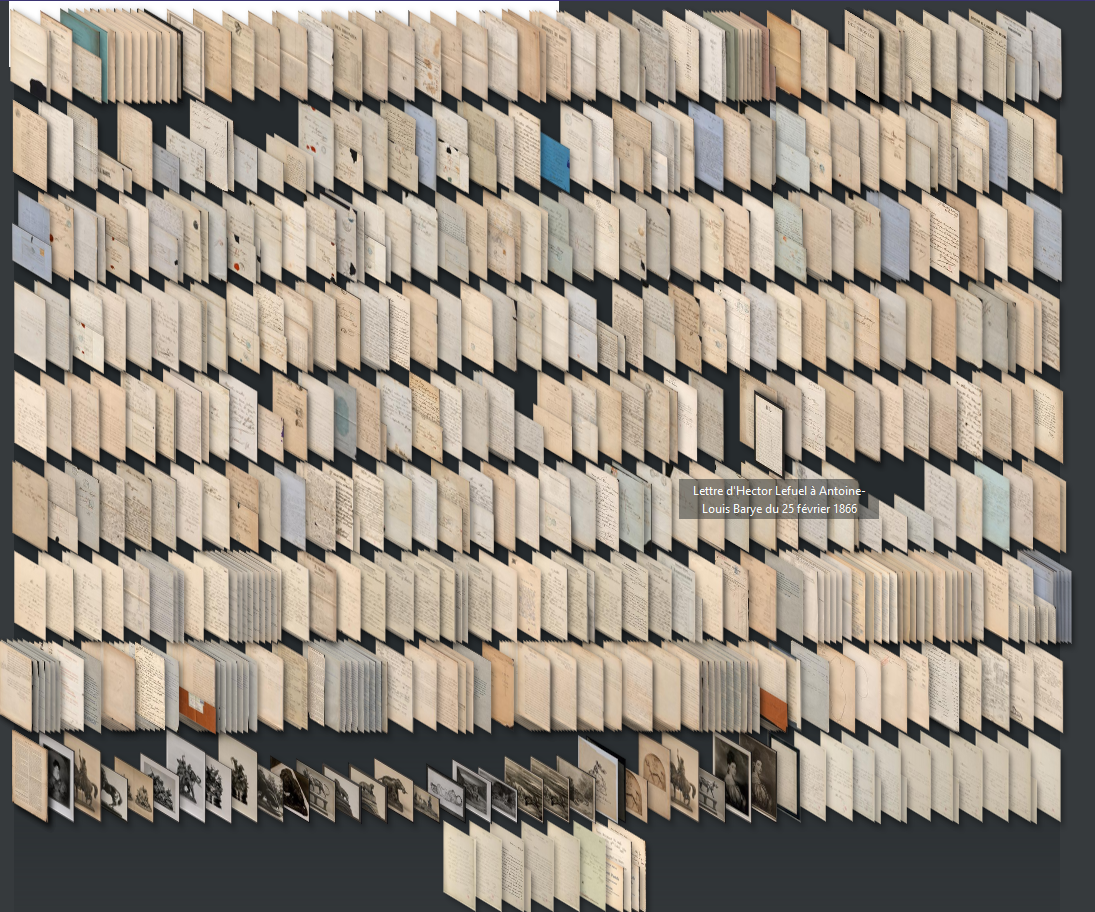
\includegraphics[width=0.8\textwidth]{barye_design_bibliotheque} 
        \caption{ Visualisation sous forme « étagère ».} 
        \label{fig:visualisation-biblio} 
\end{figure}

\begin{figure}[h] 
        \centering 
        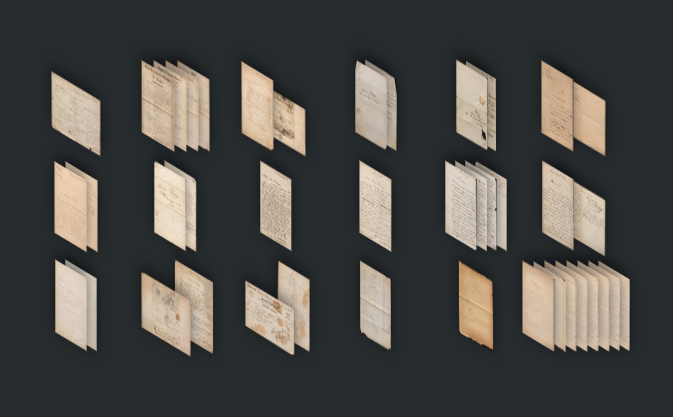
\includegraphics[width=0.8\textwidth]{barye_design_parcours_arts_deco} 
        \caption{Visualisation dite « en parcours ».} 
        \label{fig:visualisation-parcours} 
    \end{figure}

Enfin, la visualisation dite « des parcours », conçue comme une déclinaison de la vue bibliothèque, en mettant en valeur une sélection de documents selon des thématiques précises\footnote{Disponible à l’adresse suivante : https://barye.inha.fr/parcours/BaryeEtLesArtsDecoratifs}.


Le projet \pense accorde également une importance particulière à l’accessibilité de ses interfaces, en intégrant des standards web adaptés aux utilisateurs de lecteurs d’écran. Cette démarche, fondée sur les recommandations WAI-ARIA\footcite{initiative_wai_wai-aria_nodate} (\textit{Accessible Rich Internet Applications}), vise à structurer le code \html et JavaScript des pages pour permettre une navigation fluide et intelligible, y compris pour les personnes en situation de handicap\footcite{faulkner_using_2018}. 
Toutefois, à ce stade, le projet n’atteint que le premier niveau de ces bonnes pratiques, se concentrant principalement sur une structuration propre du \html en y ajoutant des attributs sémantiques, afin de permettre aux personnes utilisant un lecteur d’écran de saisir une partie de la richesse des pages.

\subsection{Projets d’édition numérique actuellement en cours (2024)}

\subsubsection{Des projets aux caractéristiques diverses}

\textbfit{Le projet Raoul-Rochette}\\

Le projet Raoul-Rochette, lancé en juin 2023, se concentre sur l’édition numérique d’un album de dessins d'art antique (essentiellement romain, étrusque et grec) constitué par Désiré Raoul-Rochette (1790-1854), archéologue et historien de l’art antique\footcite{gran-aymerich_raoul-rochette_2010}.
Ce projet a permis de constituer une base de données tiré de l’extraction de « composants » des dessins, segmentés selon différents critères (planches, dessins, signatures) grâce à l’utilisation de la plateforme Transkribus\footcite{inha_dessins_nodate}. Un prototype d’édition numérique a été mis en ligne, proposant une recherche à facette qui permet de filtrer les œuvres selon divers paramètres : le type de dessin, les matériaux représentés, l’aire chrono-culturelle, l’auteur du dessin, ainsi que les lieux de découverte et de production des objets représentés. Cette édition croise donc les données iconographiques en haute définition avec un commentaire érudit tiré des ouvrages de l’archéologue, favorisant une confrontation entre l'image et le texte, et s’inscrit en lien direct avec la bibliothèque numérique de l’INHA. 
Le projet est néanmoins actuellement en pause indéfinie à l'heure actuelle (2024).
\newline
\textbfit{Le projet Pressouyre}\\

Un autre projet significatif est celui consacré aux documents de fouille de l’archéologue Léon Pressouyre, assisté par son épouse Sylvia, historienne de l’art, dans la mise au jour des vestiges du cloître disparu de la collégiale Notre-Dame-en-Vaux (Châlons-en-Champagne), édifié au XIIème siècle et détruit à partir de 1759. 
Le projet, lancé en septembre 2023, porte sur l’étude des archives de Pressouyre (1935-2009), elles aussi conservées par l’\inha \footnote{Voir : https://calames.abes.fr/pub/\#details?id=FileId-3423}   qui documentent une entreprise de recherche et de reconstitution intellectuelle de plus de vingt ans. Ce fonds d’archives considérable, composé de carnets de notes, relevés et fichiers détaillant les fouilles entreprises à partir de 1963, sous la supervision de Pressouyre et de son équipe\footcite{inha_edition_nodate-1} est particulièrement remarquable, comme le souligne Isabelle Périchaud, coordinatrice du projet, de par le soin particulier qui a été apporté à l’inventaire rigoureux de chaque découverte, ce qui confère à ce fonds une richesse « exceptionnelle » \footcite{perichaud_a_2022}. 
Le projet, soutenu à nouveau par l’utilisation de Transkribus pour la transcription et la segmentation des fiches de fouille, vise également une modélisation en trois dimensions du cloître, à partir des fragments retrouvés. Cette approche plutôt novatrice (mais non complètement nouvelle pour \pense !) contribue à révéler un peu plus l’ambition expérimentale du projet. 
\newline
\textbfit{Le projet Thierry}\\

Un troisième projet notable est le projet Thierry, lancé en septembre 2023 et mené en collaboration avec Jérôme Delatour, responsable des collections photographiques de l'\inha, ainsi que les chercheuses Sipana Tchakerian et Nayiri Tcharkhoutian. Ce projet porte sur le fonds d'archives de Jean-Michel et Nicole Thierry, historiens de l'art (tous deux initialement de formation médicale),  spécialisés dans l'art arménien (auteurs avec Patrick Donabédian de l’ouvrage de référence publié chez Mazenod, \textit{Les arts arméniens}, 1987) \footcite{mouradian_jean-michel_nodate}, et vise à éditer et valoriser les nombreux documents rassemblés au cours de leurs voyages de recherche sur une période s’étendant sur 46 ans\footcite{inha_fonds_nodate}. 
Les archives, essentiellement des fiches de voyage, incluent des itinéraires, des commentaires et des photographies. Le travail de transcription (manuelle) et de segmentation (automatique) est en cours. Si la segmentation automatique a pu être mise en place du fait d’une certaine régularité de mise en forme notamment en ce qui concerne les fiches d’itinéraires, il est à noter qu’une transcription automatique par \ocr, a été écartée, et ce, bien que les documents soient tous quasi-intégralement typographiés, du fait de l’introduction de caractères non latins, comme des caractères de l’alphabet arménien, ainsi que d’un riche système d’abréviations complexes, qui nécessiteraient un entraînement spécifique du modèle d’\ocr pour produire des résultats satisfaisants. Le projet comporte une composante de visualisation cartographique des différents trajets effectués par les Thierry, avec une projection des itinéraires sur une carte, qui a fait l’objet d’un prototype mis en ligne\footcite{inha_fonds_nodate}. 
Pour chaque voyage documenté par les fiches, le trajet est projeté sur un fonds de carte pour l’instant vierge – un choix privilégié dans un premier temps, tant du point de vue technique (lisibilité des informations), que du point de vue scientifique (complexité de représentation de l’évolution des frontières au cours du temps et tensions politiques à prendre en compte émergeant de la dénomination choisie pour les lieux, notamment en ce qui concerne les territoires disputés encore aujourd’hui entre l’Arménie et l’Azerbaïdjan par exemple (citons le conflit au Haut-Karabakh)).
Enfin, il convient de souligner que l’un des aspects centraux de \pense réside dans la multimodalité de ses projets. Du traitement iconographique (\textit{Karbowsky}, \textit{Raoul-Rochette}) à la modélisation 3D (\textit{Karbowsky}, \textit{Pressouyre}), en passant par la cartographie interactive (\textit{Thierry}), \pense met en avant une approche fluide et hybride qui articule des disciplines et des méthodes variées.

\subsubsection{La correspondance Doucet/René-Jean, un statut à part ?}

\textbfit{La BAA et la Bibliothèque de l’INHA : un héritage institutionnel riche}\\

Le projet d’édition de la correspondance entre Jacques Doucet, couturier, collectionneur et mécène que nous avons déjà présenté, et René-Jean, proche collaborateur de Doucet, critique d’art et bibliothécaire de la Bibliothèque d’Art et d’Archéologie, s’inscrit dans le cadre du programme intitulé « La Bibliothèque d'art et d'archéologie de Jacques Doucet : corpus, savoirs et réseaux » \footcite{lequipe_du_carnet_edition_2021} lancé en 2018\footcite{noauthor_a_nodate}, peu après le déménagement de la Bibliothèque de l’\inha dans la salle Labrouste, en 2016\footcite[p.17-19]{cugy_histoire_2020}. Le projet s’appuie également sur la base de données « Acteurs de la BAA », disponible sur la plateforme AGORHA\footcite{inha_lettres_nodate}. 
Le programme, initié par Marie-Anne Sarda, est une poursuite d’un précédent programme mené de 2011 à 2016 sur les collections personnelles de Jacques Doucet, et coordonné par Chantal Georgel. Ce programme entend valoriser l’héritage institutionnel de Doucet, à travers la numérisation et l’étude de ses archives, conservées à la \bnf et à l’\inha. Le fonds principal sur lequel repose ce projet est le « NAF 13124 », constitué de la correspondance de Doucet et René-Jean, donnée à la \bnf en 1946 par René-Jean lui-même\footcite{inha_lettres_nodate}. Ce fonds constitue la majeure partie de l’ensemble documentaire faisant l’objet de l’édition numérique (89 sur les 98 documents recensés). Un fonds secondaire, « Autographes 143-145 », est conservé à la bibliothèque de l'\inha dans le fonds Doucet et est issu d’un don plus récent réalisé par la fille de René-Jean, Sylvie Maignan en 2006\footcite{flejou_jacques_2015}.

Le projet d’édition numérique de la correspondance au sein du projet \pense a débuté lui au printemps 2021 sous la direction de Pascale Cugy, historienne de l’art et spécialiste de la \baa\footcite[p.2]{cugy_histoire_2020}, parallèlement au développement du projet \textit{Karbowsky}, lui aussi en lien direct avec la figure de Doucet, nous l’avons dit. Il s’agissait pareillement de « confirmer » la réplicabilité des processus utilisés pour le fonds Barye. 

Il est tentant de considérer le projet d’édition de l’échange épistolaire de Doucet avec René-Jean, qui de par sa nature, sa temporalité et ses correspondants, aborde beaucoup la question de l’élaboration de la \baa ; comme ayant une place particulière au sein de l’institution. En effet, il existe un lien de filiation clair entre la \baa et la Bibliothèque de l’\inha, régulièrement volontiers présentée comme une « héritière » de la bibliothèque de Doucet. Rappelons que la \baa, constituée à partir de 1908 dans « 6 appartements de la rue Spontini » \footcite{flejou_jacques_2015}, toute entière consacrée à l’histoire de l’art et à l’archéologie, et constituée avec une approche voulue comme scientifique (intégrant des publications savantes, des archives, des fonds photographiques et iconographiques comme des dessins ou des estampes) a été donnée par Doucet à l’Université de Paris en 1917 puis rattachée à l’\inha en 2003. Par ailleurs, le fonds issu de la \baa de Doucet constitue encore une grande partie des collections de la bibliothèque de l’actuel \inha, comme le souligne Pascale Cugy\footcite[p.2]{cugy_histoire_2020}. 
La correspondance entre Jacques Doucet et René-Jean, qui nous permet d’explorer la manière dont Doucet entretenait ses relations avec ses collaborateurs artistiques et savants, apparait comme auxiliaire précieux pour comprendre la genèse et le fonctionnement de la \baa : il est donc tout naturel de la voir devenir objet d’une édition numérique à part entière dans le cadre de \pense. 
\newline
\textbfit{Les figures de Jacques Doucet et de René-Jean : brèves présentations biographiques}\\

Né en 1853, Jacques Doucet a d'abord bâti sa fortune dans la haute couture, reprenant le magasin familial situé rue de la Paix à Paris et le faisant connaître mondialement en y cultivant une clientèle prestigieuse. Collectionneur, amateur d’art, il s’intéresse d’abord aux collections XVIIIème (l’un des objets de l’édition \textit{Karbowsky}), avant de se tourner vers le mécénat d’artistes contemporains, notamment après la vente en 1912 de sa collection XVIIIème à la suite d’un traumatisme personnel, la mort brutale de sa maîtresse Jeanne Ruaud. Saisissant l’intérêt esthétique de l’avant-garde, il acquiert en 1924 les \textit{Demoiselles d’Avignon} de Picasso. Son très fort intérêt pour l’histoire de l’art, perceptible dans toutes ses entreprises (y compris ses choix artistiques en tant que couturier), prend forme avec la constitution d’une bibliothèque qui deviendra la \baa. Ses collections parvenues à la Bibliothèque de l’\inha en 2003 sont aujourd’hui conservées sous le fonds « Bibliothèque de l’INHA – collection Jacques Doucet ». Il disparaît le 30 octobre 1929 à l’âge de 76 ans.

René-Jean, de son nom de naissance René Hippolyte Jean (1879-1951), lui, est issu d’un milieu plus modeste. Il officie d’abord comme journaliste et critique d’art dès 1900, avant de devenir sous-bibliothécaire à la Bibliothèque des Arts décoratifs (1904). Il est finalement engagé le 1er septembre 1908 par Doucet en qualité de bibliothécaire, « plus comme collaborateur que comme fonctionnaire »\footnote{Extrait de la lettre d’engagement de Doucet à René-Jean : « […] Le plus sérieux est que vous devez à la bibliothèque que je forme tout votre dévouement et toute votre intelligence, que je considère prendre en votre personne plus un collaborateur qu’un fonctionnaire. », dans \footcite[p.139]{chapon_cetait_2006}}, avec pour mission de constituer une bibliothèque spécialisée dans l’histoire de l’art\footcite{sarda_rene-jean_2021}, la même qui deviendra plus tard la \baa. 
